\chapter{Summary.\\
Sammenvatting.\\
Perspective and Outlook} \label{ch-6}

\newpage
\section{Summary}
Most of the biological processes that maintain cellular life depend on habitually interacting proteins, forming complexes that correlate with the type of biological processes they are involved in. To better understand these processes, researchers attempt to structurally characterize macromolecular protein assemblies using numerous different biochemical and biophysical techniques. Most commonly, protein assemblies are structurally elucidated using X-ray crystallography, cryogenic electron microscopy/tomography (cryo-EM/ cryo-ET) and mass spectrometry (MS). As briefly reviewed in \textbf{Chapter 1}, each of these methods has benefits and drawbacks associated, however most of the methods predominantly require a highly purified sample. The downside being that macromolecular protein assemblies are, up to more recently, rarely studied in their naïve cellular environment. In this thesis, the versatility of cross-linking mass-spectrometry (XL-MS), to characterize protein assemblies \emph{in vivo} is demonstrated. We show that especially in mitochondria, for which cryo-ET identification is limited to the biggest or most "uniquely-shaped" complexes \cite{RN1} such as the ATP synthase (\textbf{\autoref{fig:ch6_fig1}}), XL-MS enables the sensitive identification of novel mitochondrial protein complexes.\\
Although XL-MS enables the characterization of protein complexes in their naïve cellular environment, established XL-MS workflows present drawbacks that significantly hamper an adequate structural characterization. The presence of coinciding respiratory chain protein assemblies in mitochondria \cite{RN3} for instance, prevent the confident identification of a cross-links origin and thereby an accurate structural characterization of a specific assembly. To tackle existing challenges of classical in-solution XL-MS, we therefore set out to develop a novel, easy-to use workflow (\textbf{Chapter 2}) termed in-gel cross-linking mass spectrometry (IGX-MS). IGX-MS circumvents time and sample consuming steps, and further provides a sensible solutions for differentiating cross-links obtained from co-occurring protein oligomers or complexes, leading up to an improved structural characterization. It seemingly also reduces the number of so-called overlength cross-links, which may originate from higher order (e.g. dimeric) structures.

\begin{figure*}[hbt!]
    \center
    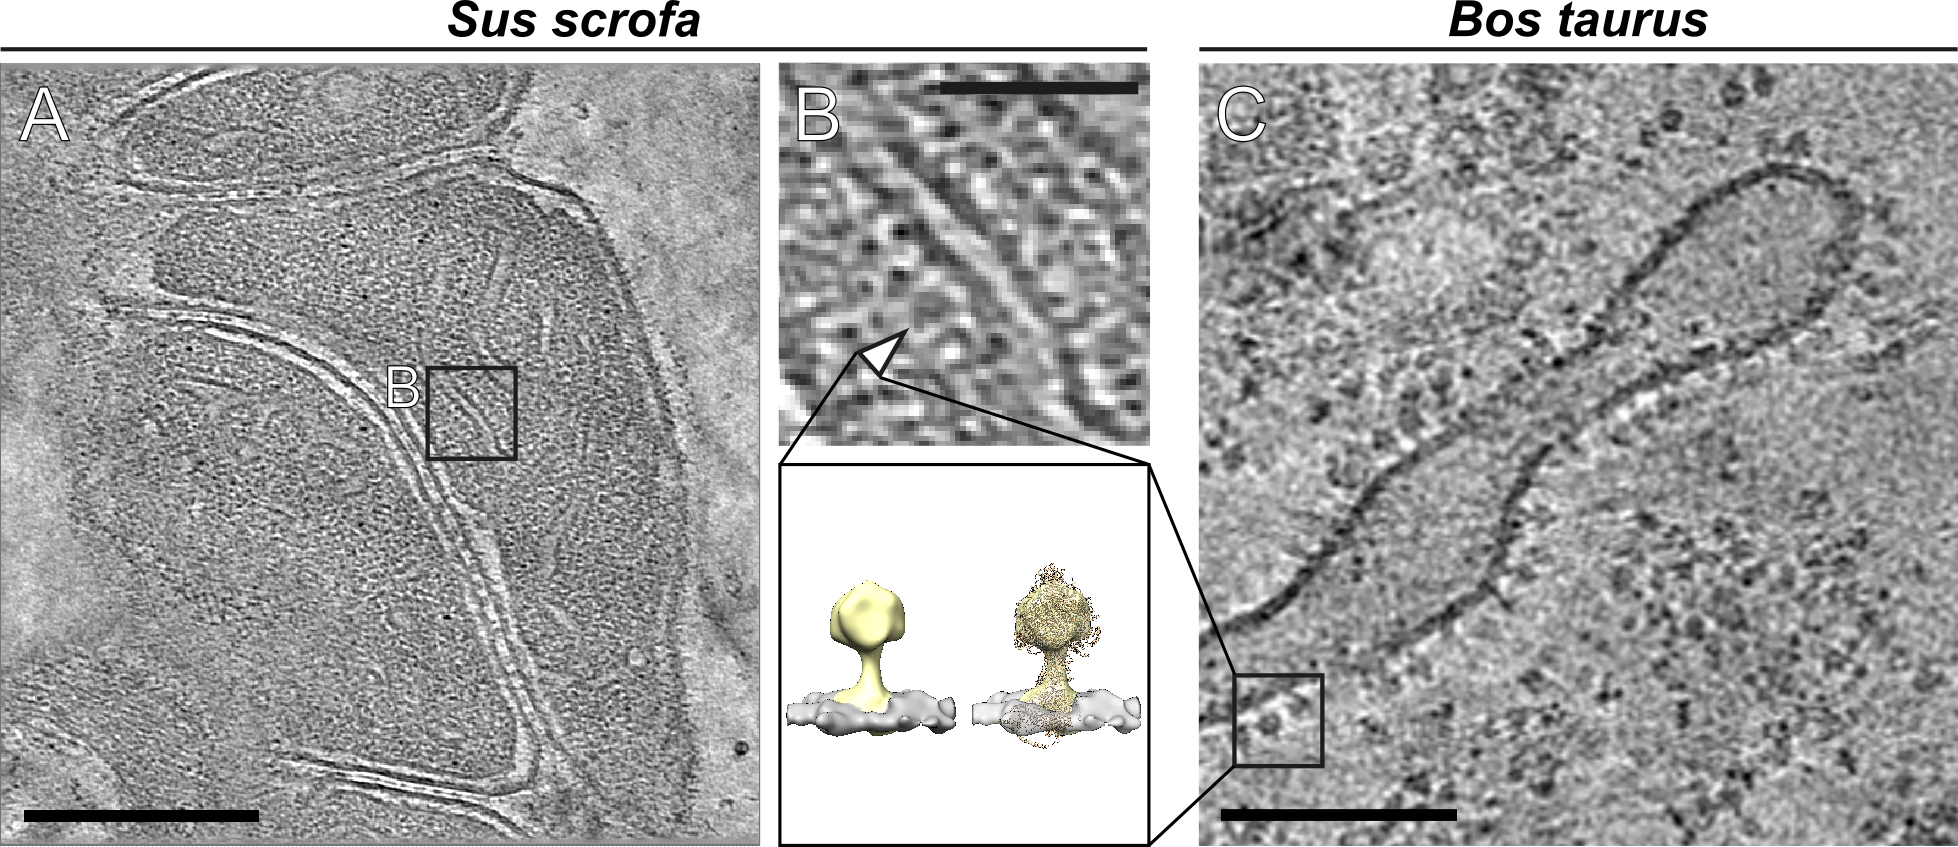
\includegraphics[width=\textwidth]{Chapter.6/Figures/Figure1.png} 
    \caption{\textbf{Cryo-electron tomography of mitochondrial membranes \emph{in vitro} and \emph{in situ}.} \textbf{A-B}. Slice through a cryo-tomogram of cryo-focused ion beam (FIB)-milled Sus scrofa sperm mitochondria. \textbf{C.} Slice through a cryo-tomogram of purified inner mitochondrial membranes from Bos taurus heart mitochondria. For both samples, ATP synthase can be directly identified based on its characteristic shape. Scale bars: A. 250 nm, B-C. 100 nm. Figure (panel A-B) adjusted from \cite{RN2} with permission. Cryo-tomogram shown in panel C was recorded and provided by Miguel Ricardo Leung (Utrecht Univresity, not published).}
    \label{fig:ch6_fig1}
\end{figure*}

In view of IGX-MS relying on BN-PAGE, unambiguous characterization of complexes requires prior knowledge about the respective apparent mass and for complex samples is limited to high abundant complexes.\\
Nevertheless, in case no prior knowledge is available or the complex of interest is low abundant, a structural characterization is still possible. Combining XL-MS with complementary structural techniques, e.g. complexome profiling (CP-MS) or cryo-ET enabled us to identify and structurally characterize novel and low abundant protein complexes in mitochondria (\textbf{Chapter 3-5}). By performing XL-MS and CP-MS for the structural analysis of macromolecular protein assemblies in bovine heart mitochondria (\textbf{Chapter 3}), we showcase that combining both techniques provides unexpected insights into the macromolecular organization of the mitochondrial interactome. Focusing on complexes of oxidative phosphorylation, XL-MS and CP-MS uncover that a substantial amount of dimeric apoptosis factor 1 (AIFM1) is associated with at least 10\% of monomeric cytochrome c oxidase (COX). Combining XL-MS and CP-MS did provide useful complementary information, demonstrating that it can be used to define and characterize multiprotein assemblies in detail, even for complexes that may have been overlooked in earlier studies, e.g. due to their low abundance, instability in detergents or \emph{in vitro}.\\
Likewise, technical limitations still hamper an adequate characterization of protein complexes in a naïve environment. As briefly described in (\textbf{Chapter 1}) and earlier in this summary, cryo-ET has emerged as powerful technique to characterize macromolecular protein assemblies \emph{in situ}, however currently being limited to a sub-nanometer resolution which often does not allow the unambiguous structural characterization of complexes. In a collaborative effort, we showcase that the current technical limitations can be overcome by additionally performing XL-MS experiments (\textbf{Chapter 4}). Using sub-tomographic averaging, the Zeev-Ben-Mordehai group (Utrecht University) identified that in mammalian sperm, mitochondria are wrapped around the flagellar cytoskeleton. It further appeared that anchoring to the cytoskeleton is mediated through ordered protein arrays consisting of boat-shaped particles on the outer mitochondrial membrane. Due to limited resolution these densities could not be unambiguously assigned, for which we were asked to support respective structural characterization by performing additional XL-MS experiments. To our delight, XL-MS provided structural constraints to further identify these densities as conserved arrays of glycerol kinase-like proteins, highlighting the advances of combining XL-MS and cryo-ET for the structural reconstruction of protein assemblies.\\
Although it enables the accurate prediction of protein structures and interactions, the experimental characterization of proteins and their complex structures is a time-consuming, highly complex and costly process. Recent breakthroughs in computer-aided structural modeling, facilitated the quick prediction of a wide variety of complex protein structures based solely on the amino acids sequence present \cite{RN5, RN4}. Although the overall prediction accuracy is high, models of e.g. proteins with only a small number of sequence homologs can have low accuracies at times, for which having additional experimental restraints at hand can be extremely valuable to validate and further refine respective models. Following up on this, I describe in \textbf{Chapter 5}, how combining XL-MS in combination with AlphaFold2 \cite{RN4} can be utilized to identify and structurally characterize giant protein assemblies (MDa) in mitochondria. Like described in \textbf{Chapter 3}, XL-MS and CP-MS data is used for the detailed characterization of mitochondrial protein assemblies, providing essential information regarding complex members and assembly state prior to structural modeling. Combining data from both methods enabled us to identify MRPS36 as a novel component of the 2-oxoglutarate dehydrogenase complex (OGDHC), and subsequently was utilized to refine the AI-driven structural model. The final model of the complete eukaryotic OGDHC has a size of $\sim$3.45 MDa and provides new insights into the topology of this multi-component enzyme as well as details on its enzymatic function. Phylogenetic analysis further revealed that MRPS36 is a key component of OGDHC, exclusively present in eukaryotes.

\section{Perspective and Outlook}
More than a decade after the initial introduction and following upon various advancements in chemistry, sample preparation, instrumentation and bioinformatics, cross-linking mass-spectrometry (XL-MS) has developed into a mature method for the structural characterization of proteins and multi-protein complexes as reviewed in \cite{RN8, RN7, RN6}. By enabling the structural characterization of proteins in a cellular context, XL-MS now provides improved opportunities to investigate a protein`s biological function and role from a structural perspective and in relation to its neighboring environment. The ever-increasing improvements in instrumentation, cross-linking reagents, experimental designs and software solutions are continuously pushing the boundaries of XL-MS into unforeseen spheres. In the following sections I am aiming at giving a broader perspective on XL-MS and its future implications.

\begin{figure*}[hbt!]
    \center
    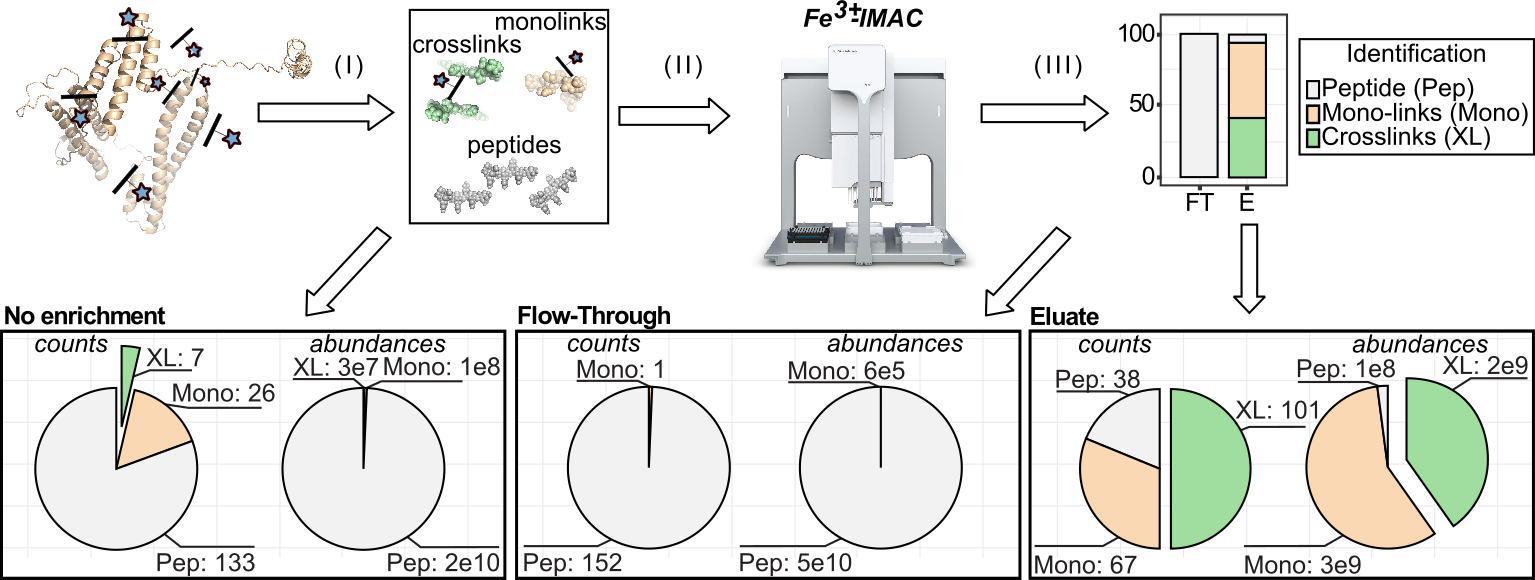
\includegraphics[width=\textwidth]{Chapter.6/Figures/Figure2.png} 
    \caption{\textbf{Workflow, and performance of an enrichable cross-link reagent (PhoX).} After cross-linking, the proteins are denatured, reduced, alkylated, and digested into peptides (I). The mixture of peptides contains 3 different kinds of products: unmodified peptides (gray), monolinks (orange), and cross-links (green) (II); these colors are reused. Cross-linked and monolinked peptides are enriched e.g. using Fe3+-IMAC on a liquid sample handling platform providing high sample throughput. Direct measurement of the cross-linked peptides produces low counts of cross-link identifications due to their extremely low abundances (left panel), while measurement following Fe3+-IMAC enrichment results in no cross-link identifications in the flow-through with similar abundance levels for the linear peptides as detected in the No enrichment (middle panel) and many in the eluate due to their enhanced abundance levels (right panel). Figure and legend adapted with permission from \cite{RN4}.}
\label{fig:ch6_fig2}
\end{figure*}

\subsection*{Improving the effectiveness of protein - protein cross-linking}
As vividly shown in this thesis but also by others \cite{RN11, RN9, RN10} cross-linking can be a powerful and successful methodology to probe proteins and protein complexes \emph{in-vivo} and \emph{in-vitro}. Notwithstanding, its effectiveness has long been impeded by interference caused by the low abundance of cross-linked peptides, especially in complex samples \cite{RN12}. A promising direction of development regards advancing from “difunctional” cross-linkers to a “trifunctional” design, e.g. by additionally including an enrichable handle (besides the two reactive moieties). Such a handle enables the selective enrichment of cross-linked peptides, thereby reducing sample complexity and ultimately enhancing MS detection (\textbf{\autoref{fig:ch6_fig2}}). Trifunctional cross-linkers were recently introduced for both, gas-phase cleavable and not-cleavable linkers, utilizing azide or alkyne tags (e.g. azide/alkyne-A-DSBSO) \cite{RN13} or a phosphonic acid (PhoX, not cleavable; \textbf{\autoref{fig:ch6_fig2}}) \cite{RN14} as enrichment handle. While the azide/alkyne-A-DSBSO reagent can be enriched via click chemistry \cite{RN15} (e.g. utilizing a biotin-conjugated alkyne/ azide probe), PhoX cross-linked peptides can be simply enriched by immobilized metal affinity chromatography (IMAC), a fast and highly robust strategy that is well established in almost all proteomic laboratories (\textbf{\autoref{fig:ch6_fig2}}).\\
Besides the low abundance of cross-linked peptides, also impaired membrane permeation ability, e.g. like observed for PhoX, can drastically, hamper XL-MS experiments. The development of cross-link reagents with improved cell permeation ability, hold therefore high potential to further improve the \emph{in-vivo} characterization of protein assemblies. A modified PhoX reagent (tBu-PhoX) \cite{RN16} was recently introduced, which utilizes a tert-butyl protection group to shield the negative charge of the enrichment handle (phosphonic acid), thereby increasing its membrane permeability \cite{RN16}. After the cross-linking reaction, the protection group is removed by an acid cleavage (e.g. TFA), allowing the enrichment cross-linked peptides via the now unprotected phosphonate handle. Another recourse for improving effectiveness of XL-MS experiments might be offered by increasing the cross-linking density. To date, the standardly used homobifunctional, NHS-reactive cross-linkers, limit the cross-linking density and conclusively the efficiency by their incapability to capture residue proximity beyond Lysine-Lysine pairs \cite{RN6}. The development of cross-link reagents with increased residue selectivity, such as the recently introduced heterobifunctional cross-link reagent sulfosuccinimidyl 4,4`-azipentanoate (sulfo-SDA) \cite{RN17} and succinimidyl diazirine sulfoxide (SDASO) \cite{RN18}, hold therefore the capacity to increase XL-MS density. Sulfo-SDS comprises a NHS ester group that interacts with primary amines (Lysine) and a diazirine group that efficiently reacts with any amino acid side chain or peptide backbone upon photo activation (330nm - 370nm) \cite{RN17, RN19, RN20}. Furthermore, photo reactive cross-linkers open up a complete new opportunity of characterizing a proteins function by additionally being able to capture protein-RNA \cite{RN21} and protein-glycan \cite{RN22} interactions. Especially protein-glycan cross-linking, with the capability of deciphering cellular glycan binding events, might help researches to investigate the potential use of glycans and glycan binding proteins as therapeutic targets \cite{RN23}. Notwithstanding, due to the complex chemical space, as well an even lower abundance of each cross-linked peptide caused by the low specificity, analysis and identification of such cross-links is highly challenging \cite{RN24, RN18}. In the future, further development needs to be implemented to facilitate the identification of respective cross-linked products. Introducing appropriate scores and statistics could help to address site-ambiguity, while investigating opportunities to specifically could simplify mass spectrometry based identification.\\
Lastly, on a more general note, increased cross-linking efficiency may also be achieved by developing novel methodologies that aim at further simplifying the identification of cross-linked peptides, e.g. by developing MS based acquisition strategies that specifically target cross-linked peptides. Likewise, constant advances in data analysis pipelines as well as improved False Discovery Rate (FDR) strategies will further benefit the field by increasing the reliability of obtained data. Lastly, as observed for many of the “younger” methodologies, XL-MS still lacks defined protocols for the execution and analysis of XL-MS experiments. Defining best practice guidelines to conduct experiments, data analysis but also unifying generated software output would drastically benefit the field by assisting researchers to generate reproducible and re-usable XL-MS results.

\subsection*{Quantitative cross-linking}
Another auspicious direction of development regards the (relative) quantification of cross-linked peptides, enabling the detection of changes observed for assembly- and conformational states, e.g. resulting from perturbations caused by a drug treatment or a disease state. Promising results have already been reported by Bruce and co-workers \cite{RN25}, who introduced a isotope labeled crosslink reagent, enabling a reliable quantification of cross-link peptides originating from different samples. Like in standard quantitative proteomics, also a label-free strategy, which can be performed with all commercially available cross-linkers, was introduced as reviewed in \cite{RN26, RN27}. For label-free quantification, MS1 signals of individual cross-linked peptides are most commonly integrated over their chromatographic elution profile. Although the high relevance to understand functional states of proteins and protein assemblies, probing structural dynamics by quantitative cross-linking approaches is still not standardly applied. While isotope-labeled cross-linkers are mostly limited to pairwise comparisons, the low abundant nature of cross-linked peptides significantly complicates the label-free MS1 based quantification. Likewise, the lack of automated quantification tools are restricting the frequent usage of quantitative XL-MS \cite{RN27}. Introducing novel workflows, e.g. utilizing tandem mass tags (TMT) for the MS2-based quantitation as shown recently in a proof of concept study \cite{RN28} or performing more targeted MS approaches e.g. data independent acquisition (DIA) \cite{RN29} or parallel reaction monitoring (PRM) \cite{RN30}, seem to be a promising path to towards a reliable quantitation of cross-linked peptides.

\subsection*{Combining XL-MS with complementary approaches to improve the structural characterization of protein assemblies}
As shown in this thesis, combining XL-MS with other techniques can highly benefit the accuracy and reliability of the characterization of protein complexes. Especially the likely ever increasing complexity of studied systems, eventually requires to find complementary approaches, which aim at facilitating the structural characterization. Within the structural proteomics toolbox (briefly reviewed in \textbf{Chapter 1}) various methods exist, that upon combination likely hold the potential to address intrinsic limitations each technique by itself may oppose.\\
A major limitation of XL-MS for the analysis of protein assemblies includes that assessing complex stoichiometries and interaction modules is highly challenging. Additionally to CP-MS, used for the work in my thesis, native MS is a highly sensitive methodology to probe assembly- and functional states of protein complexes as reviewed in \cite{RN31}.
Accordingly, it was already highlighted that a combination of both methods works extremely well for purified, soluble complexes \cite{RN32, RN33}, but complex systems have not been challenged so far. Notwithstanding, recent breakthroughs in native MS, e.g. a study showing the ejection of assemblies directly from native membranes \cite{RN34}, open up new possibilities to further characterize more complex systems like membrane embedded protein complexes.\\ 
The structural characterization of membrane embedded proteins and protein complexes might be of particular interest as it lags far behind their soluble counter parts \cite{RN35, RN36}, although their significant clinical relevance e.g. drug development \cite{RN37}. While XL-MS to date is mostly limited to soluble accessible residues, methods that provide additional information membrane embedded interfaces are needed. Besides native MS, thermal proteome profiling (TPP) might also be a highly complementary technology to XL-MS. Briefly, TPP detects changes in the thermal stability of proteins, which can be affected upon the interaction with other proteins \cite{RN38}. Like so, TPP can reflect the complex architecture of membrane proteins \cite{RN38}, providing additional information about membrane embedded interfaces that are not susceptible to XL-MS. Moreover, detected protein-protein interactions can be used to additionally validate protein complexes identified with XL-MS.\\
Like TPP, limited proteolysis MS (LiP-MS) is able to detect changes that might not be susceptible to XL-MS. LiP-MS relies on a sequential tryptic digestion step with a non-specific protease being applied under naïve conditions prior to a complete tryptic digestion under denaturing conditions \cite{RN39, RN40}. This enables the identification of protein structural changes on peptide level after perturbation (e.g. drug treatment, change of nutrients, etc.) \cite{RN41}, thereby providing additional information (e.g. drug targets or metabolite binding sites) which would not be accessible with XL-MS due to for instance its residue selectivity. Combining XL-MS with LiP-MS might therefore hold the potential to provide a more complete picture regarding the structural features of a protein or protein complex, in that improving respective functional characterization.\\
Besides combining XL-MS with other mass spectrometry based techniques, the combination with well-established structural techniques such as X-ray crystallography and electron microscopy holds great potential to aid the structural characterization. The benefits of utilizing XL-MS in conjunction with cryo-electron microscopy (cryo-EM) and cryo-electron tomography (cryo-ET) have been already reviewed in detail \cite{RN43, RN42, RN44} and are also illustrated by work described in this thesis (\textbf{Chapter 4}). In brief, especially sample heterogeneity and protein flexibility can drastically hinder higher resolution in single particle cryo-EM, for which restraints from XL-MS are extremely useful to validate and guide model building as shown for the investigation of the architecture of the Mad1:C-Mad2 complex \cite{RN45}. In this study, XL-MS data is used to assess the conformation and flexibility of the Mad1:Mad2 complexes in solution, highlighting that in solution Mad1:Mad2 adopts variable conformations with a preferred tendency to adopt a folded rather than an elongated state (\textbf{\autoref{fig:ch6_fig3}}).\\

\begin{figure*}[hbt!]
    \center
    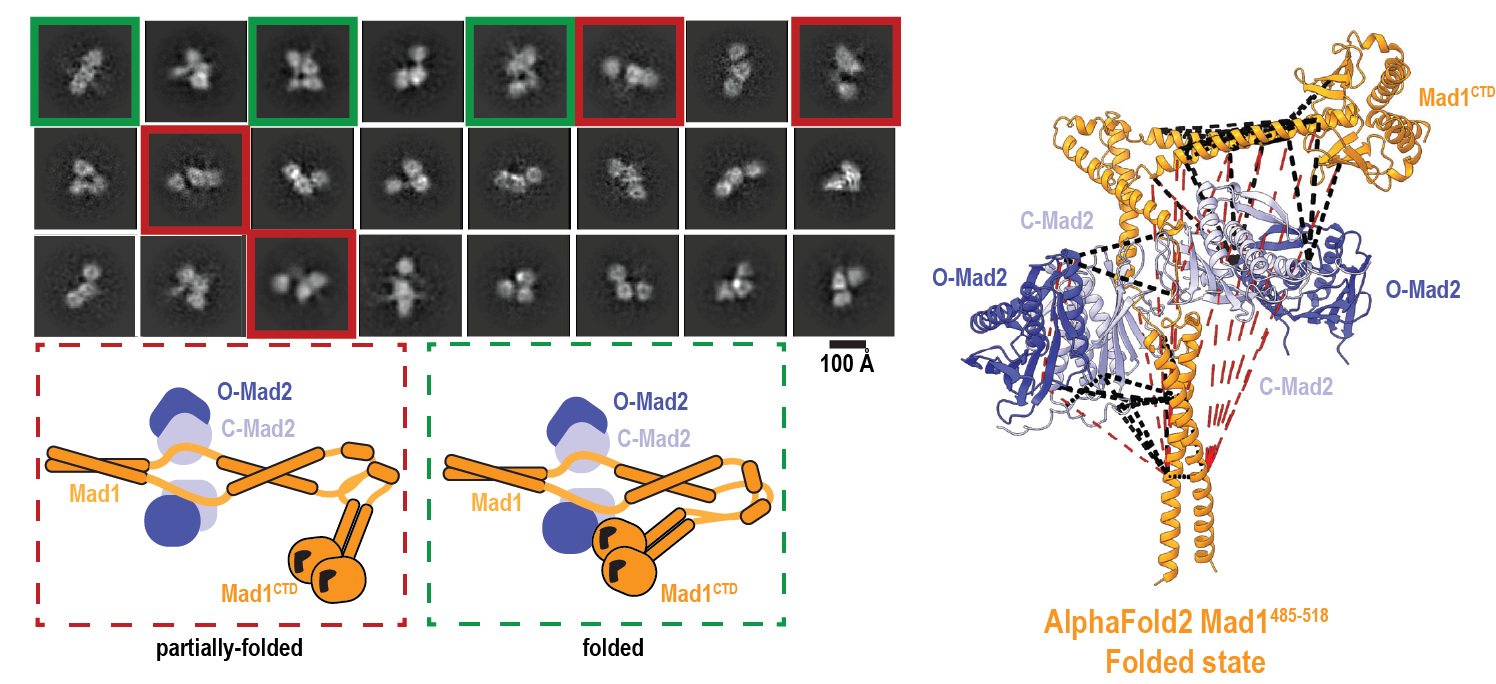
\includegraphics[width=\textwidth]{Chapter.6/Figures/Figure3.png} 
    \caption{\textbf{A folded state of the Mad1:Mad2 complex.} Representative 2D averages of BS3 cross-linked pMad1:C-Mad2:O-Mad2 complex by cryo-EM (left panels). Classes showing complexes that appear only partially folded are boxed in red, and classes showing complexes that appear fully folded are boxed in green. A schematic of the suggested partially folded and folded states seen in the 2D averages is shown below. XL-MS was used to confirm folded state (right panel). An AlphaFold2 predicted model of the folded hexameric Mad1:C-Mad2:O-Mad2 complex was validated using identified cross-links. Mad1 subunits (residues 485-718) are shown in orange, whereas C-Mad2 and O-Mad2 are coloured in light and dark blue, respectively. Mapped cross-links with a distance below 40 Å are indicated as black dashed lines and all others in red. For all obtained cross-links, only the shortest option is depicted. Figure adapted with permission from \cite{RN45}.}
\label{fig:ch6_fig3}
\end{figure*}
\clearpage

Lastly, as pointed out in the introduction of this thesis (\textbf{Chapter 1}), and as illustrated in (\textbf{Chapter 5}) restraints from XL-MS are highly valuable for the computational modeling of proteins and protein complexes by either restraining the possible conformational space or by offering an additional scoring feature for generated models. The recent success of AI driven de novo protein structure prediction \cite{RN5, RN4}, enables the generation of structural models based solely on a proteins amino acids sequence. Although the overall prediction accuracy is high, models can have low accuracies at times for which a careful validation is needed. Integrating XL-MS data as additional restraints into the modeling pipeline can improve the accuracy of the generated models, e.g. by guiding the domain or subunit positioning as well as supporting the model refinement. Further, mapping identified cross-links onto generated models would provide an additional layer of validation, facilitating the process of finding the most accurate model.\\

Altogether, the versatility that is provided by XL-MS alone, but also in conjunction with other MS based or structural techniques is growing, thereby expanding its applicability. Ultimately, in my view XL-MS is well on the way to become an indispensable methodology to decipher large, heterogeneous and highly flexible protein complexes \emph{in-vivo}. 

\clearpage
\section*{References}
\bibliographystyle{Style_settings/bibstyle_pnas}
\bibliography{Chapter.6/chapter6_bib}
